\newpage
\section{Independent Q-Learning}\label{sec:IQL}
Q-Learning is an off-policy temporal difference control algorithm. Temporal difference methods can learn directly from raw experience without a model of the environment's dynamics. Furthermore, it updates estimates based in part on other learned estimates, without waiting for a final outcome \cite[pp. 133]{RL1}. 

While the distinguishing feature of on-policy methods is that they estimate the value of a policy while using it for control, these two functions are separated in off-policy methods. The behavior policy, used to generate behavior, and the estimation policy, that is evaluated and improved, may in fact be unrelated. This separation is an advantage because the estimation policy may be deterministic (e.g., greedy), while the behavior policy can continue to sample all possible actions \cite[pp. 126]{RL1}. Its simplest form, \emph{one-step Q-learning}, is defined by \cite[pp. 148]{RL1}:
\begin{align*}
Q(s_t,a_t) & \leftarrow Q(s_t,a_t) + \alpha \left[ r_{t+1} + \gamma \displaystyle\max_a Q(s_{t+1},a) - Q(s_t,a_t) \right]
\end{align*}
When using Q-Learning in a multi-agent setting independently for each agent, the method is called Independent Q-Learning (IQL). In IQL, for a single agent, all the other agents are modeled as part of the environment. While Q-Learning is guaranteed to converge, Independent Q-Learning is not guaranteed to converge. This is because the premise of the convergence porperty of Q-Learning is that the environment be stationary. This will not be the case in a multiagent setting in which agents are learning concurrently, since the agents base their policy upon the movements of the other agents which are also learning. That is, the other agents don't act deterministically but are modeled as such. Independent Q-Learning can thus not be justified theoretically \cite[pp. 57]{vlassis}.

\subsection{Implementation}
For this assignment, we implemented Independent Q-learning and used it independently for all our agents, the predators and the prey. The agents learn concurrently (i.e. all agents do a move, then all update their estimated values), not sequentially (i.e. after one agent does a move, all other agents update their estimated values). When any two predators bump into each other, the prey wins (reward of $10$) and the predators all lose (reward of $-10$). When a predator catches the prey, the prey loses and all predators win.

 Each agent will have its own state representation and learning and will view the other agents as part of the environment. We used $\epsilon$-greedy action selection, which behaves greedily most of the time, but with probability $\epsilon$, instead select an action at random, uniformly, independently of the action-value estimates \cite[pp. 28]{RL1}. In this case, we used $\epsilon = 0.1$. We initiated the values of each Q-learning table optimistically with a value of 15 for all cells for the tables.

\subsubsection{State space} \label{sec:stateSpaceIQL}
The state space is of crucial importance to Independent Q-Learning, because it grows exponentially with the number of agents. In the experiments described in the previous report, were we had just one prey and one predator, we initially used a state space that was an intuitive, yet cumbersome representation. We then changed the state space representation to a more efficient one in the second assignment, referred to as the `efficient' state space, which led to a reduction of 697 times less states, resulting in just 21 different states. See Section \ref{sec:stateSpaceIntro} for details.

The default amount of states for this assignment would be $121^{p+1}$ for each agent, where p equals the number of predators. By using the efficient state space this has been reduced to $21\cdot 121^{p-1}$ because the prey's position is fixed in the state space representation and the predator to which this state space belongs moves along those $21$ states, the rest is used to determine in which state the predator currently resides. In this assignment however the prey also learns, so to make use of our state space representation, a single predator will be used as reference point every time so that the predator is fixed at the position $(0, 0)$ in our state space and the prey would be moving around the $21$ states just like a predator. 

The reduction is increased further by pointing to the same state for each combination of current positions of the other predators, though this is only effective for more than two predators. A simple example would be a case three predators and a prey, the current predator ($p_1$) which has to find his current state would take the position of the first other predator ($p_2$) and then the position of the second other predator ($p_3$) to locate his state in the state space. In this case it shouldn't matter which position, $p_2$ or $p_3$, would be looked up first. In this case both $p_2$ then $p_3$ and $p_3$ then $p_2$ would point to the same state. This reduces the state space to:

\[
\mathbf{stateSpaces}(p) = 
\begin{cases}
	21 & p = 1\\
    21 \cdot 121 & p = 2 \\
    \frac{21\cdot 121^{p-1}}{(p-1)!}& p > 2
\end{cases}
\]


\subsection{Results}

We analyzed what happened in the case of 2, 3 and 4 predators.
We did not analyze what happens in the case of there being one predator, because we already analyzed that in our previous report and there is no difference between Q-Learning and IQL for the case of  one prey and one predator.

However, even when using this efficient state space representation we ran out of time while trying to initialize one prey and four predators for the $11 \times 11$ grid world. We dedicated around $3.6$ GB heap space for the JVM on a $64$-bit machine with $4$ processor cores of $2.67$ Ghz, and under these settings it took more than $7$ hours to declare and initialize four predators, the prey not being created and initalized yet.
However, when using a $9 \times 9$ grid world instead of a $11 \times 11$ one, the five agents were swiftly up and running. 
Therefore we will show the results for $2$,$3$ and $4$ predators for this $9 \times 9$
 grid world first, and later we will attempt to make a comparison with the $11 \times 11$ grid world.



\subsubsection{Number of predators}

\begin{figure}[hbt]
\centering
%bb = llx, lly, urx, and ury;
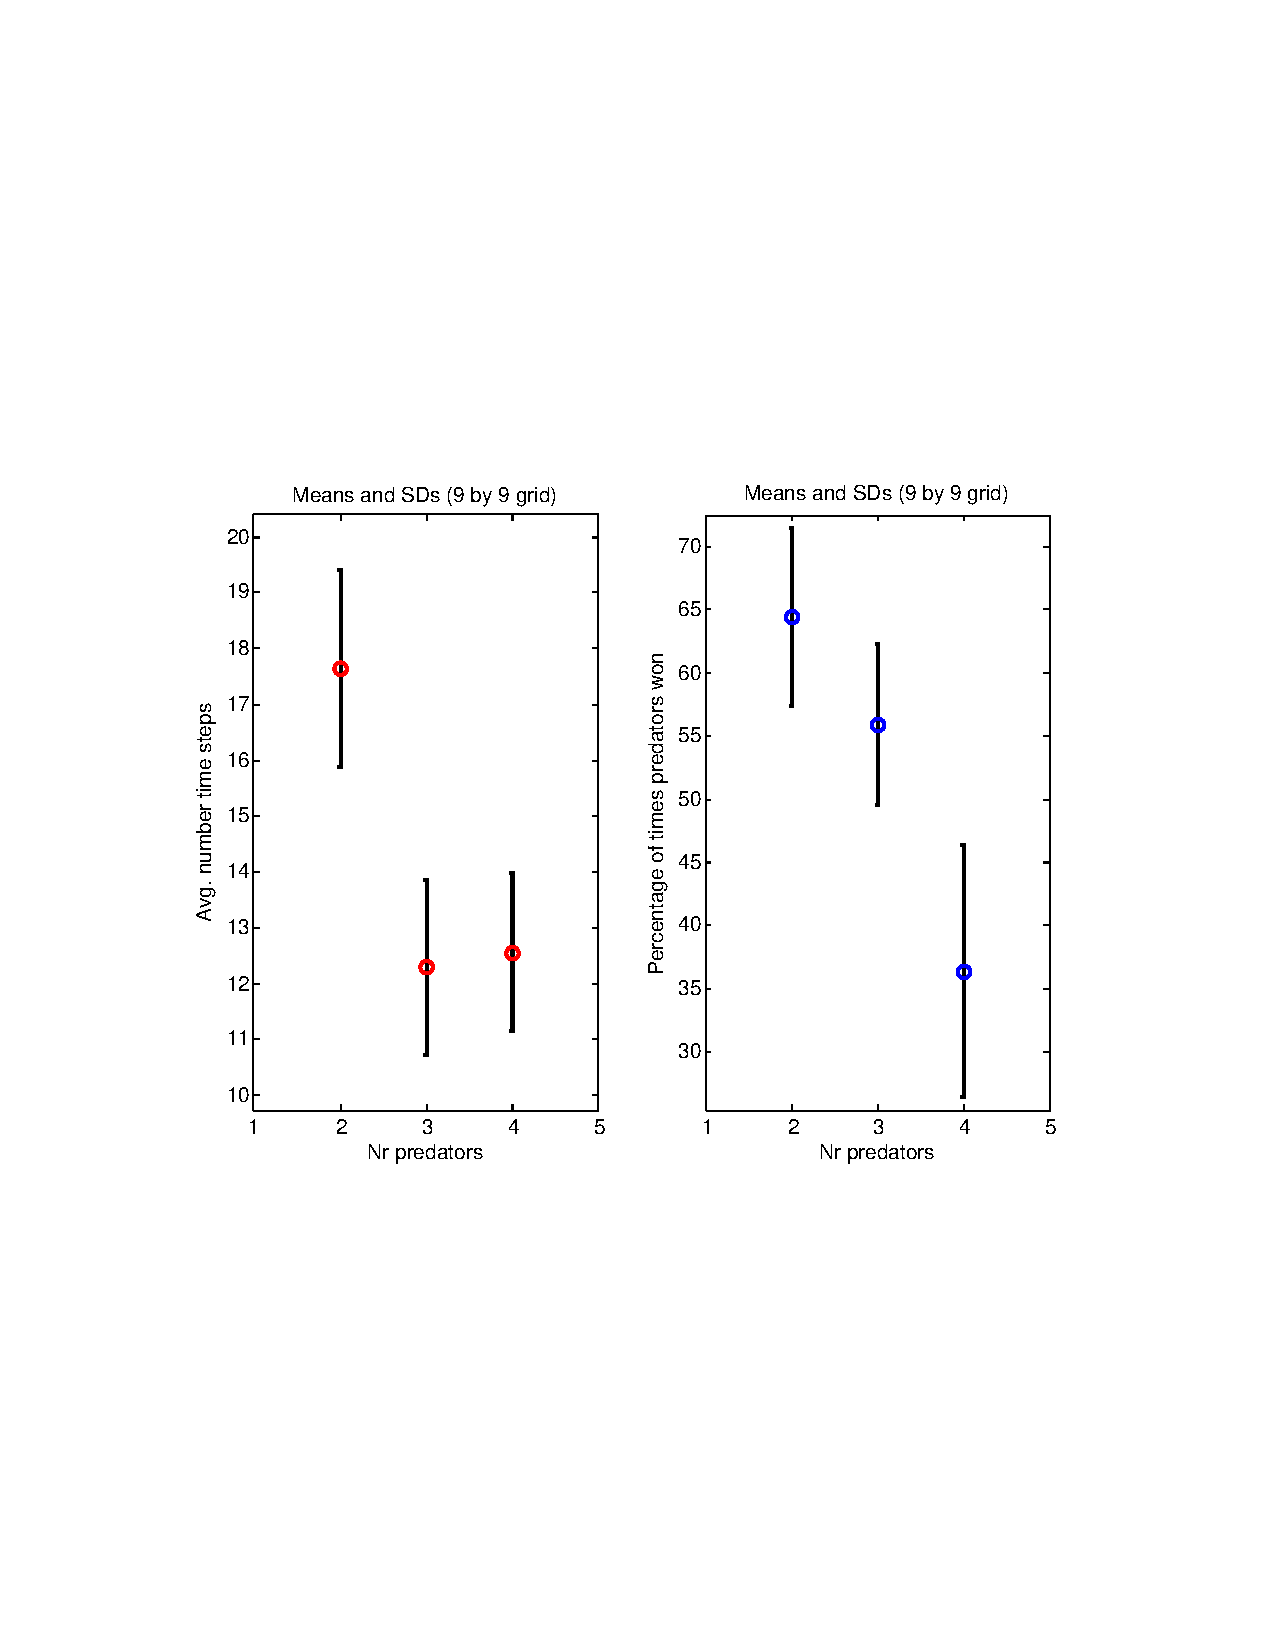
\includegraphics[bb = 0.6in 3in 7.9in 8.5in,clip,width=0.7\textwidth]{IQLgrid9by9ErrorBars.pdf} 
\caption{Error bar plot of performance in a 9 $\times$ 9 grid}
\label{fig:meansSds}
\end{figure}

\FloatBarrier


\subsubsection{Using an 11 $\times$ 11 grid}



\begin{figure}[hbt]
\centering
%bb = llx, lly, urx, and ury;
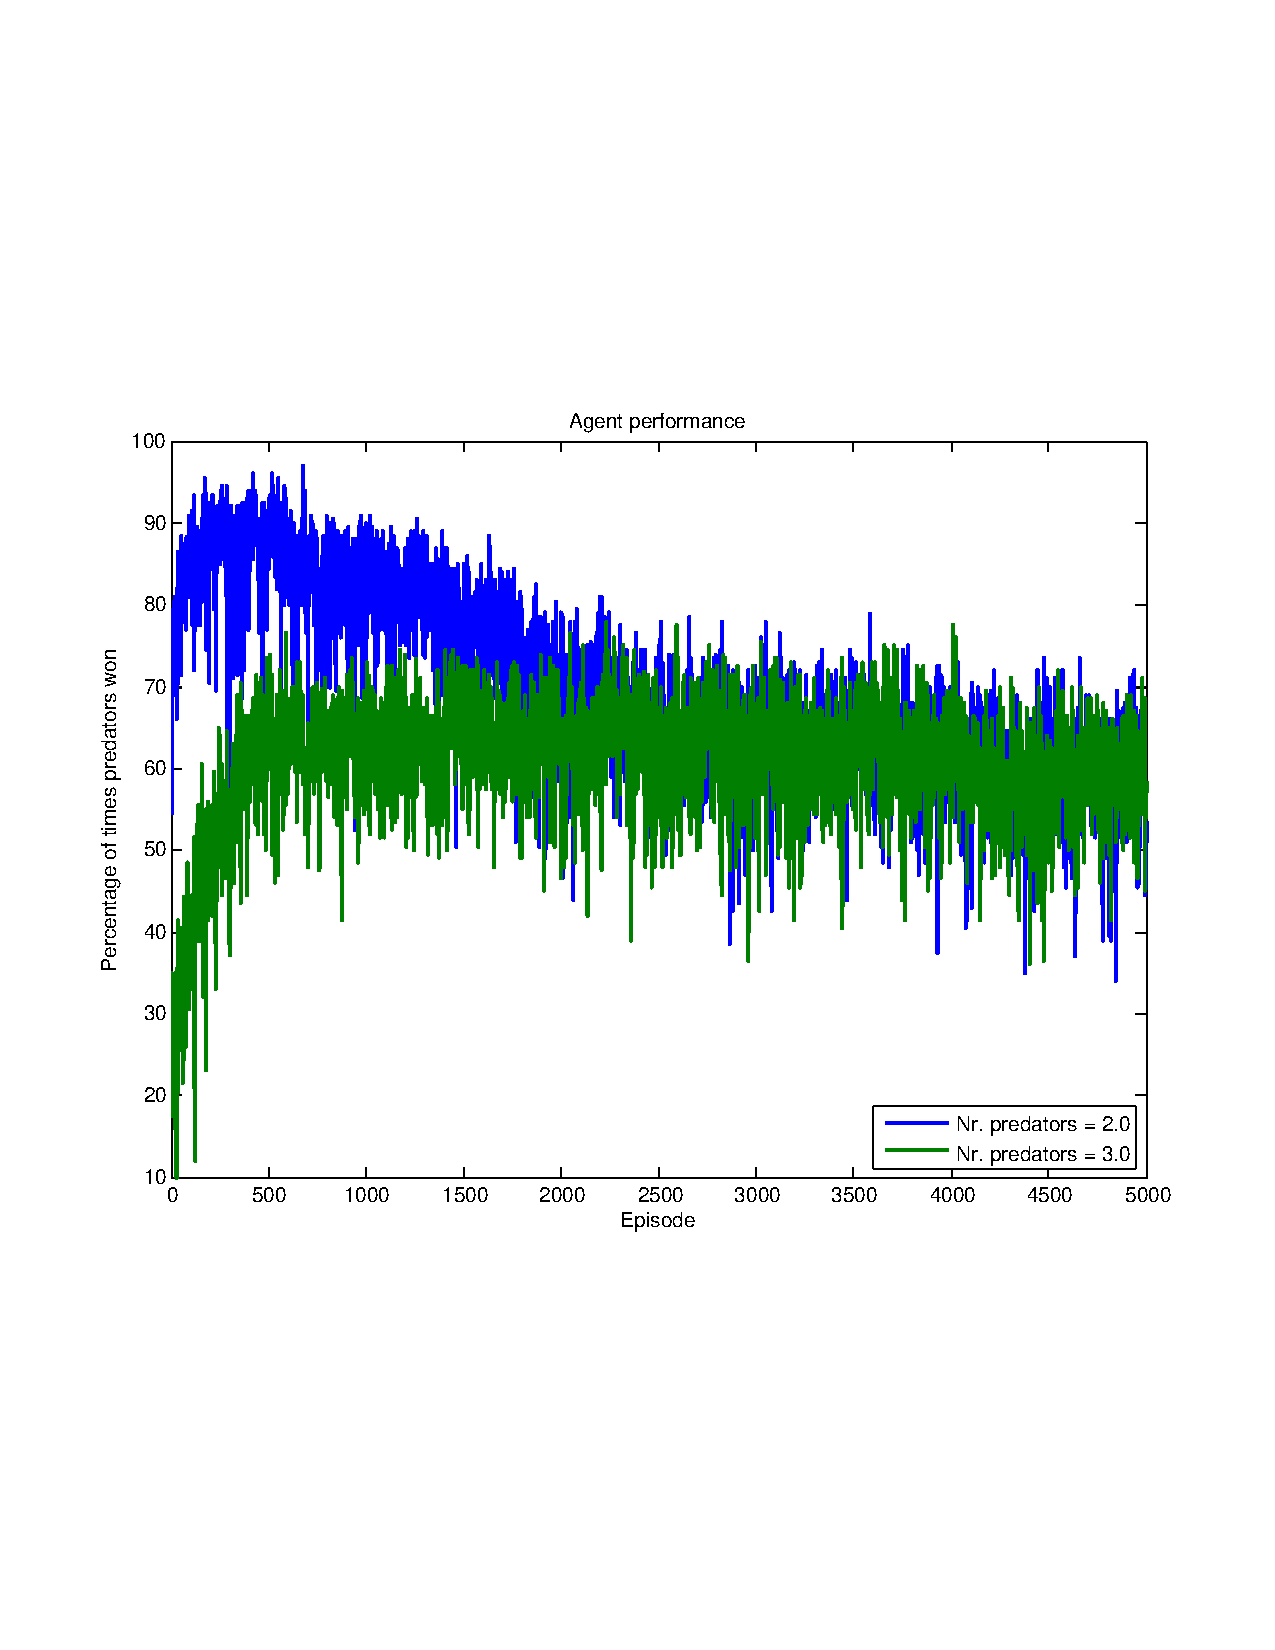
\includegraphics[bb = 0.6in 3in 7.9in 8.5in,clip,width=0.7\textwidth]{IQLpercentageWinning5000episodesavg200trials.pdf} 
\caption{Bla}
\label{}
\end{figure}

\FloatBarrier

